\chapter{La aplicación de asignación promedio}\label{ch:5}

En este capítulo se comparan dos tipos de aplicaciones de asignación diferentes: la aplicación de asignación de máxima entropía, construida en la sección \ref{sec:maxentcons}, y la \textit{aplicación de asignación promedio}.

\section{Definición y acercamiento}

Nos interesamos en este capítulo en la \textit{asignación de aplicación promedio} \cite{Macro-To-Micro}. Esta aplicación asigna a un estado efectivo $\rho_{\ef} \in \densityspace{n}$ un estado microscópico $\varrho_{\avg} \in \densityspace{m}$ que es una mezcla estadística de estados finos. Más específicamente, le asigna el promedio del conjunto de todos los estados puros microscópicos tales que son compatibles con el estado efectivo bajo una aplicación de grano grueso en particular (dada por la ecuación \ref{eq:CG}). Dicho conjunto de estados puros microscópicos queda definido como
\begin{equation}\label{eq:Omega}
    \Omega_{\mcC}(\rho_{\ef}) = \{\ket{\psi}\in\hilbert_{m}:\, \mcC(\dyad{\psi}) = \rho_{\ef}  \}.
\end{equation}
La aplicación de asignación promedio es el promedio sobre dicho conjunto, \ie 
\begin{equation}\label{eq:AvgMap}
    \mcA_{\mcC}^{\avg}(\rho_{\ef}) = \overline{\Omega_{\mcC}(\rho_{\ef})} = \int d \mu\,\, \delta(\mcC(\dyad{\psi})-\rho_{\ef})\,\dyad{\psi},
\end{equation}
donde $d\mu$ es la medida de Haar sobre los estados puros de $\hilbert_{m}$. La delta de Dirac asegura que únicamente se tomen en consideración a los estados puros compatibles, y la medida de Haar, que la integración sobre dicho conjunto sea uniforme. Dicho de otra forma, la aplicación de asignación promedio da por hecho dos cosas sobre el sistema microscópico: que puede estar estar en un estado puro, y que todos los estados puros son igualmente probables.

La solución analítica a la ecuación (\ref{eq:AvgMap}) es complicada y no se discutirá en este trabajo, pero ha sido encontrada por los doctores C. Pineda y R. Uriostegui del Instituto de Física de la UNAM, para el caso en que la aplicación de grano grueso va de $\densityspace{4}$ a $\densityspace{2}$\footnote{Debido a que el trabajo no ha sido publicado aún, no hay una referencia disponible.}. Esto es, del espacio de dos partículas de dos niveles, al espacio de una partícula de dos niveles. Aquí no se profundizará en dicho resultado, pero se utilizará para poder comparar ambas aplicaciones de asignación.

\section{La diferencia entre asignaciones}

Aunque las hipótesis de la aplicación de asignación promedio puedan parecer razonables, Jaynes, en su artículo, argumenta que estas son tan arbitrarias como cualquier otra suposición, a menos que algún tipo de simetría del sistema sugiera lo contrario. Nos preguntamos sobre la diferencia entre el estado de máxima entropía y el estado promedio, como una función del parámetro $p_{1}$ de la aplicación de grano grueso (recuérdese que en el caso $n=1$ el segundo parámetro es simplemente $(1-p_{1}$)) y del radio de Bloch del estado efectivo inicial $r_{\ef}$, \ie{} 
\begin{equation}\label{eq:DistAvgMaxEnt}
    \text{d}_{F}\qty(\avgass(\rho_{\ef}),\maxass(\rho_{\ef}))=\text{d}_{F}\qty(\avgass(\rho_{\ef}),\maxass(\rho_{\ef}))(p_{1},r_{\ef}),\nonumber
\end{equation}
donde $\text{d}_{F}(A,B)$ designa a la distancia entre dos matrices inducida por la norma de Frobenius. La norma de Frobenius de una matriz $A$ es
\begin{equation}
  \norm{A}_{F}=\sqrt{\Tr(AA^{\dagger})},\nonumber
\end{equation}
de tal forma que
\begin{equation}
  \text{d}_{F}(A,B)=\norm{A-B}_{F}.\nonumber
\end{equation}
Como se mencionó previamente, la expresión de $\avgass(\rho_{\ef})$ no es sencilla, así que esta distancia se analizará de manera cuantitativa. La figura \ref{ap:DistAvgMaxEnt} muestra dicha distancia, primero como función del parámetro de ruido $p_{1}$ para diferentes valores del radio de Bloch del estado efectivo inicial, $r_{\ef}$, y luego como función de $r_{\ef}$ para diferentes valores de $p_{1}$.
\begin{figure}[ht!]
    \centering
    \begin{subfigure}{0.5\textwidth}
      \centering
      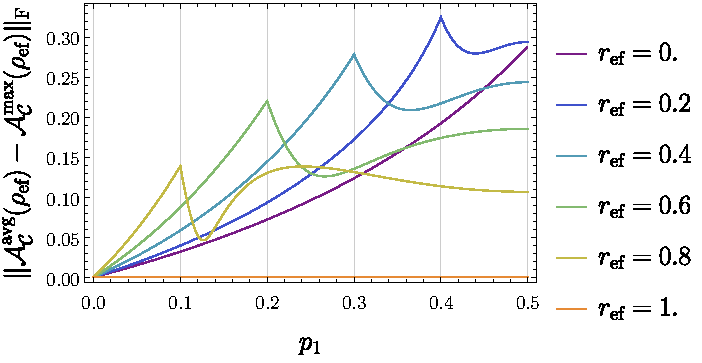
\includegraphics[width=1.\linewidth]{chapter5/figures/dist_maxent_avg_vs_p.pdf}
    \end{subfigure}%
    \begin{subfigure}{0.5\textwidth}
      \centering
      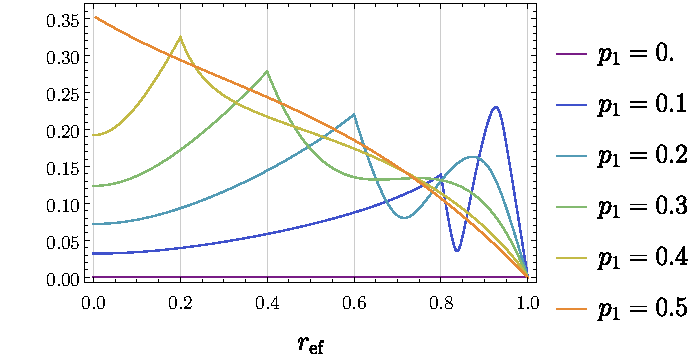
\includegraphics[width=1.\linewidth]{chapter5/figures/dist_maxent_avg_vs_z.pdf}
    \end{subfigure}
    \caption{Distancia de Frobenius entre asignaciones como función de $p_{1}$ para diferentes valores de $r_{z}$, y como función de $r_{z}$ para diferentes valores de $p_{1}$.}\label{ap:DistAvgMaxEnt}
\end{figure}

Lo primero que puede observarse en dichas gráficas es que la distancia no es diferenciable para valores de $r_{\ef}$ y $p_{1}$ tales que $r_{z}=1-2p_{1}$. Esta característica es una consecuencia del comportamiento de la asignación promedio, y no de la asignación de máxima entropía. Para convencerse de esto basta con observar la figura \ref{ap:DistAvgMaxEntId}, que muestra las distancias de Frobenius de la asignación de máxima entropía y de la asignación promedio al estado máximamente mezclado.
\begin{figure}[ht!]
    \centering
    \begin{subfigure}{0.5\textwidth}
      \centering
      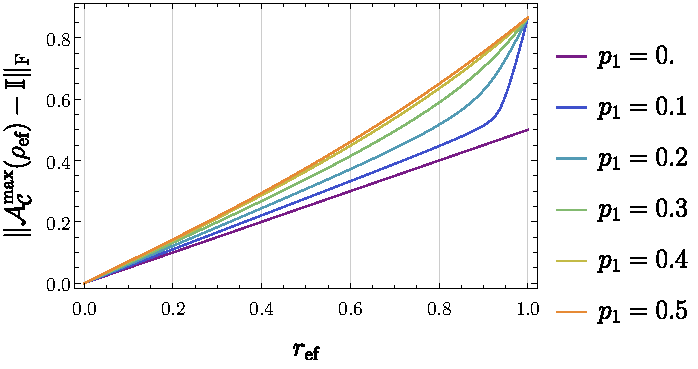
\includegraphics[width=1.\linewidth]{chapter5/figures/dist_maxent_or_vs_p.pdf}
    \end{subfigure}%
    \begin{subfigure}{0.5\textwidth}
      \centering
      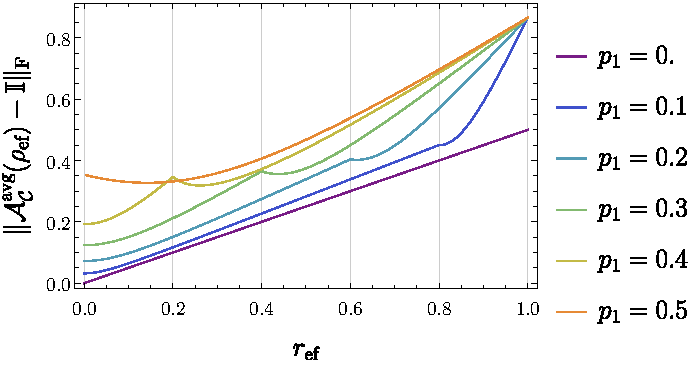
\includegraphics[width=1.\linewidth]{chapter5/figures/dist_avg_or_vs_p.pdf}
    \end{subfigure}
    \caption{Distancia entre asignaciones y el estado máximamente mezclado.}\label{ap:DistAvgMaxEntId}
\end{figure}

De las figuras \ref{ap:DistAvgMaxEnt} y \ref{ap:DistAvgMaxEntId} se puede extraer información interesante. Por un lado, hay dos casos en los que las asignaciones son iguales. El primero siendo el caso en el que el estado efectivo inicial es puro, \ie{} $r_{\ef}=1$. Este resultado ya había sido previamente discutido y demostrado: de acuerdo con la ecuación (\ref{eq:PureEffectiveState}), $\avgass(\rho_{\ef})=\maxass(\rho_{\ef})=\rho_{\ef}\otimes\rho_{\ef}$. El segundo siendo el caso en que la aplicación de grano grueso se reduce a una traza parcial ($p_{1}\in\{0,1\}$), para el que el estado asignado en ambos casos es $\Id\otimes\rho_{ef}$ o $\rho_{\ef}\otimes\Id$. Por otro lado, mientras que la asignación de máxima entropía asigna al estado máximamente mezclado $\Id_{2}/2$ el estado máximamente mezclado correspondiente, $\Id_{4}/4$, la asignación promedio no hace esto.

Las diferencias y similitudes entre las asignaciones tendrán efectos en las dinámicas efectivas. Recordando que el estado efectivo evolucionado está dado por la composición
\begin{equation}
    \rho_{\ef}(t)=(\mcC\circ\mcE_{t})(\mcA_{\mcC}(\rho_{\ef}(0))),\nonumber
\end{equation}
es natural que siempre que $\mcA_{\mcC}^{\max}(\rho_{\ef}(0))=\mcA_{\mcC}^{\avg}(\rho_{\ef}(0))$ coincidan, entonces $\Gamma_{t}^{\avg}=\Gamma_{t}^{\max}$. Sin embargo, como hemos visto, las asignaciones no suelen coincidir.


\section{Comparación de dinámicas efectivas}

Ahora que se ha definido a la aplicación de asignación promedio y que es claro que en general no coincide con la aplicación de máxima entropía, podemos comparar la dinámica emergente asociada a cada aplicación de asignación. Como el objeto principal del presente escrito era la asignación de máxima entropía, y porque los resultados que se obtienen de la asignación promedio deben ser estudiados de manera cualitativa, sólo se analizarán dos dinámicas: la dinámica local simétrica, y la compuerta de cómputo cuántico SWAP. La primera restringida al caso de dos partículas.

\subsection{Dinámicas locales}

\subsubsection{Dinámica local simétrica}

Consideramos la unitaria local simétrica
\begin{equation}
    \mcU_{t}=U_{t}\otimes V_{t},\nonumber
\end{equation}
donde $U_{t},V_{t}\in\unitaryspace{2}$ y $U_{t}=V_{t}$. Debido a que el promedio es lineal, la dinámica simétrica se factoriza cuando se utiliza la aplicación de asignación promedio. Para ver esto, nótese que
\begin{equation}
  U_{t}\otimes U_{t}=(\Id\otimes U_{t})(\varrho_{\avg})(\Id\otimes U_{t}^{\dag}).\nonumber
\end{equation}
Luego, descomponiendo al estado efectivo evolucionado en la base de las matrices de Pauli,
\begin{align}
  \rho_{\ef}(t)=\frac{1}{2}\sum_{j=0}^{3}\Tr\qty[\pauli{j}\rho_{\ef}(t)]\pauli{j} & & \text{con} & &\Tr\qty[\pauli{j}\rho_{\ef}(t)]=\Tr\left\{\pauli{j}\mcC\qty[\mcU_{t} (\varrho_{\avg}) \mcU_{t}^{\dagger}]\right\}.\nonumber
\end{align}
Como $\Tr\qty[(A\otimes \Id) \varrho]=\Tr\qty[ \Tr_{2}(\varrho)]$ y gracias a la propiedad cíclica de la traza es inmediato que la dinámica efectiva es
\begin{equation}
    \Gamma_{t}^{\avg}(\rho_{\ef})=U(t)\rho_{\ef}(U(t))^{\dag}.\nonumber
\end{equation}
Por lo que, en este caso, las dinámicas gruesas coinciden.

\subsubsection{Dinámica general}

Debido a que la aplicación promedio crea correlaciones que la aplicación de máxima entropía no, la dinámicas efectivas generadas por una evolución local no coinciden en general, como lo demuestran las figuras \ref{ap:EffDunAVGvsMaxEnt1} y \ref{ap:EffDunAVGvsMaxEnt2}.

\begin{figure}[ht!]
    \centering
    \begin{subfigure}{0.5\textwidth}
      \centering
      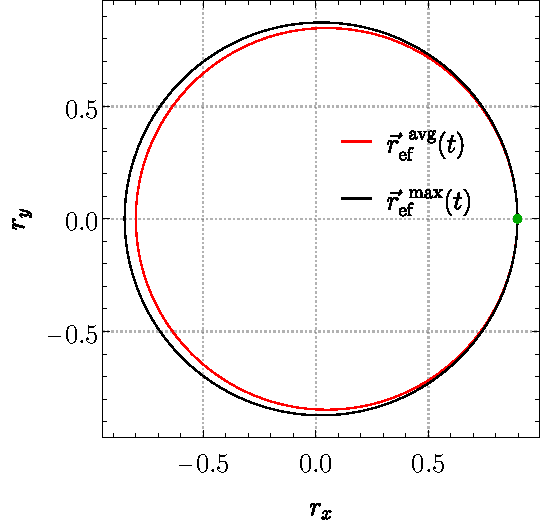
\includegraphics[width=0.8\linewidth]{chapter5/figures/local_AvgVSMax_p2=0.1_r=0.9_w1=0_w2=1.pdf}
      \caption{$H=\Id\otimes\pauli{3}$}
    \end{subfigure}%
    \begin{subfigure}{0.5\textwidth}
      \centering
      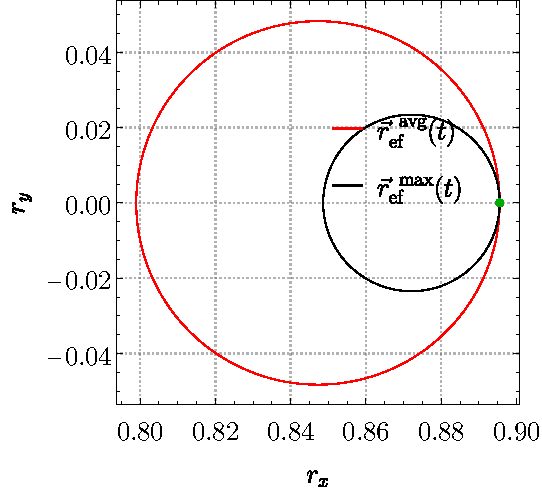
\includegraphics[width=0.8\linewidth]{chapter5/figures/local_AvgVSMax_p2=0.1_r=0.9_w1=1_w2=0.pdf}
      \caption{$H=\pauli{3}\otimes\Id$}
    \end{subfigure}
    \caption{Variaciones correspondientes a la dinámica efectiva inducida por diferentes hamiltonianos en un sistema de dos partículas partiendo de un estado efectivo inicial (verde) tal que $r_{\ef}=0.9$ y $r_{z}\approx0.09$. En rojo, la evolución del estado promedio. En negro, la del estado de máxima entropía. \label{ap:EffDunAVGvsMaxEnt1}}
\end{figure}

\begin{figure}[ht!]
    \centering
    \begin{subfigure}{0.5\textwidth}
      \centering
      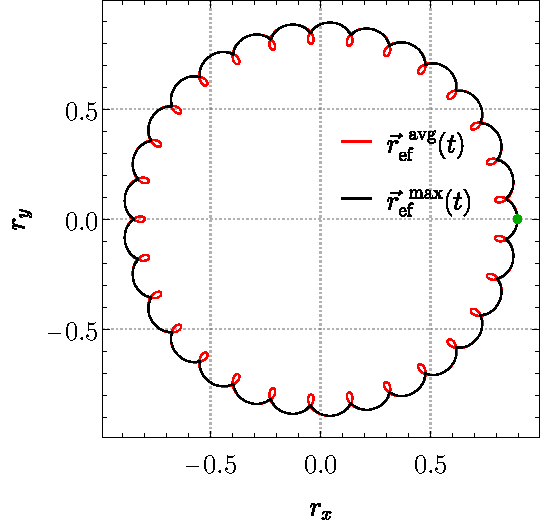
\includegraphics[width=0.8\linewidth]{chapter5/figures/local_AvgVSMax_p2=0.1_r=0.9_w1=30_w2=1.pdf}
      \caption{$H=30\pauli{3,1}+\pauli{3}$}
    \end{subfigure}%
    \begin{subfigure}{0.5\textwidth}
      \centering
      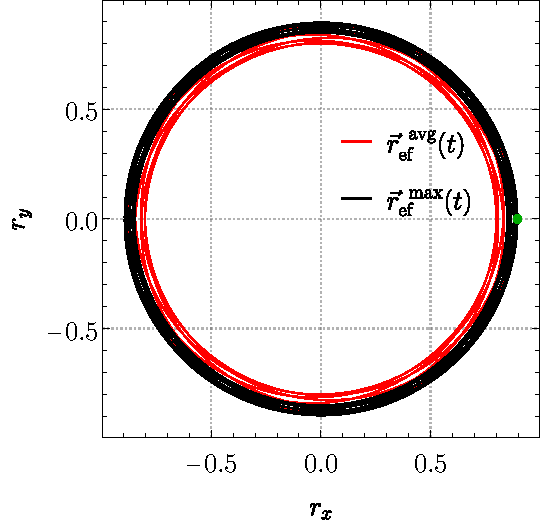
\includegraphics[width=0.8\linewidth]{chapter5/figures/local_AvgVSMax_p2=0.1_r=0.9_w1=1_w2=10.pdf}
      \caption{$H=\pauli{3,1}+10\pauli{3}$}
    \end{subfigure}
    \caption{Variaciones correspondientes a la dinámica efectiva inducida por diferentes hamiltonianos en un sistema de dos partículas partiendo de un estado efectivo inicial (verde) tal que $r_{\ef}=0.9$ y $r_{z}\approx0.09$. En rojo, la evolución del estado promedio. En negro, la del estado de máxima entropía. \label{ap:EffDunAVGvsMaxEnt2}}
\end{figure}

Debido a que la aplicación de asignación promedio únicamente toma en cuenta estados puros, la contribución del entrelazamiento es más importante. Esto conduce a una mayor pérdida de información bajo la aplicación de grano grueso y, como consecuencia, una mayor contracción en la esfera de Bloch, que es lo que podemos observar en las figuras \ref{ap:EffDunAVGvsMaxEnt1} y \ref{ap:EffDunAVGvsMaxEnt2}.

\subsection{La compuerta SWAP}

La dinámica efectiva generada por la compuerta cuántica SWAP y la aplicación de asignación promedio es, de manera similar a como ocurrió cuando se utilizó la aplicación de asignación de máxima entropía, un canal de despolarización. Estos canales de despolarización coinciden de forma trivial cuando las asignaciones lo hacen, esto es, para $p_{1}\in\{0,1\}$ y también cuando $r_{\ef}=1$. Sin embargo, resulta que las dinámicas coinciden también cuando $p_{1}=\frac{1}{2}$. Aún más, la dinámica es la misma independientemente de la asignación que se escoja. Sea $\rho_{\ef}(0)\in\densityspace{2}$ el estado efectivo inicial y $\varrho=\mcA(\rho_{\ef}(0))$ un estado compatible bajo la aplicación de grano grueso cuando $p_{1}=\frac{1}{2}$. La dinámica efectiva:
\begin{align}
  \Gamma_{t=1}^{\mcA}(\rho_{\ef}(0))=&\mcC\qty[S\varrho S]\nonumber\\
  =&\Tr_{2}\qty[S\qty(\frac{1}{2}\varrho+\frac{1}{2}S\varrho S)S]\nonumber\\
  =&\Tr_{2}\qty[\frac{1}{2}S\varrho S+\frac{1}{2}\varrho ]\nonumber\\
  =&\rho_{\ef}(0)\nonumber
\end{align}
Esto es, toda la esfera de Bloch es invariante bajo la dinámica efectiva inducida por una evolución microscópica SWAP si el parámetro de la aplicación de grano grueso es $p_{1}=\frac{1}{2}$. Fuera de estos casos particulares, el canal de despolarización efectivo no es necesariamente el mismo cuando se usan diferentes aplicaciones de asignación.

\subsection{Discusión}

La geometría del espacio de $2$ qubits es relativamente complicada \cite{JAKOBCZYK}. Esto hizo de la resolución de la integral (\ref{eq:AvgMap}) un problema no trivial. Aún más, la aplicación de asignación promedio no es fácilmente escalable a sistemas de $n$ qudits\footnote{En oposición al qubit, que es un sistema cuántico de dos niveles, un qudit es un sistema cuántico de $d$ niveles. Actualmente, los qudits son estudiados como alternativa a los qubits \cite{qudit}}. Por otro lado, como se mostró en la sección \ref{sec:maxentcons}, utilizar el Principio de Máxima Entropía permite dichas extensiones de forma directa (la extensión a qudits, aunque no se desarrollará aquí, se logra utilizando una base adecuada del espacio de operadores hermitianos que actúan sobre $\hilbert_{d^{n}}$). Esto abre un camino directo a la obtención de resultados analíticos, cosa que se ha aprovechado en el presente escrito. 

En caso de no haber una razón para incluir únicamente estados puros en la definición de la aplicación de asignación promedio, esta restricción es tan arbitraria como considerar que todos los estados microscópicos compatibles con el estado efectivo son igualmente probables (suposición que también se hace). La elección de los estados a considerar, así como la medida sobre la que realizar la integración, son elementos de información que inyectan un sesgo a los resultados que puedan ser obtenibles. La aplicación de asignación de máxima entropía utiliza únicamente la información accesible al observador, y puede ser modificado para incluir nuevas restricciones. 